\label{chap-intro-ds}

\label{intro-DS}

Distance sampling (\cite{IDS}, \cite{ADS}) is a popular method for estimating the abundance of biological populations. It has been used by researchers across the globe to assess the abundance of everything from birds nests to marine mammals. Surveys are cheap to run since they do not require many observers (unlike a census) or multiple site visits (unlike mark-recapture). Distance sampling is also rather different from methods like mark-recapture (\cite{ruthbook}) as it does not explicitly include the abundance in the likelihood, as shall be seen below. The popularity of distance sampling is in part due to the software Distance (\cite{distance-software}) which makes it easy to record and analyse distance sampling data. 

\section{From quadrat sampling to distance sampling}

One can think of distance sampling as the logical extension of quadrat and strip transect sampling. In quadrat sampling a series of squares (quadrats) are laid out at random over the sample area and the number of objects of interest within each is counted. It is assumed that within each quadrat a census is performed. From the per-quadrat abundance the density is estimated and multiplied-up to find the total abundance. For quadrat sampling to be efficient the quadrats need to be large and hence it is almost impossible to ensure that all objects in the quadrat are seen, this can be further hindered by animals moving between the quadrats during the survey (\cite[p. 2]{IDS}).

% evolution to DS from quadrat and strip
\begin{figure}
\centering
% trim order l b r t
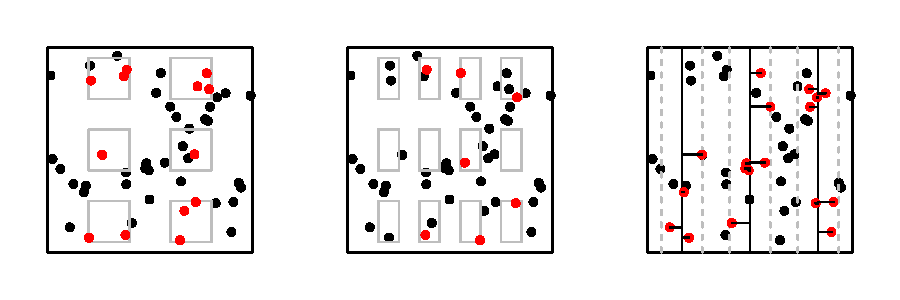
\includegraphics{intro/figs/quadrat-to-ds.pdf}\\
\caption{An example of quadrat sampling (left), strip transect sampling (middle), and distance sampling (right). Dots indicate individuals, red dots are observed individuals, black those missed. In the first two cases, the grey boxes represent the sampling units. Note that there are many observations just outside of the boxes, which cannot be recorded by survey staff. In the distance sampling case, the solid vertical lines represent the transects and the dashed line gives the effective strip width. Distances are shown by the solid horizontal lines.}
\label{quad-to-ds}
\end{figure}

To make the task of counting the objects within the quadrat easier, one could modify the square design to be a long strip, so that the observer could walk down the centreline of the strip, observing those objects within the strip. Mathematically, if we let the each strip be of width $2w$ ($w$ either side of the line the observer walks down) and the sum of all strip lengths be $L$, if $n$ objects are observed we have a simple estimator of the density, $D$:
\begin{equation}
\hat{D}=\frac{n}{2wL}.
\label{ds-simpleD}
\end{equation}

The problem with both quadrat and strip sampling is that there may well be many objects just outside of the covered area. Clearly this is a waste of survey effort, since observers must ignore objects that they have seen but that are not within the strip. It would be preferable to include as many observations as possible and leverage the maximum amount of data that can be collected to assess the abundance of the population.

Distance sampling is based on this principle; if the objects of interest are seen, then their presence should be recorded. Instead of using fixed-area sampling units, distance sampling requires that only centrelines are specified. The observers should walk (or swim, ride, drive, sail, etc) down the centrelines recording the distances ($x_i$) to the observed objects as they go. Once the survey is complete, the distances are used to estimated the effective area that was sampled. Figure \ref{quad-to-ds} shows the evolution from quadrat to strip to distance sampling.

In equation (\ref{ds-simpleD}) one can think of replacing $w$ with an estimate of $\mu$, the \textit{effective strip (half-)width}. This is the distance at which as many animals were detected beyond as there were missed inside. Further explanation of $\mu$ is given in \secref{gtoD}, but it serves for now to say that by replacing $w$ with $\mu$, an estimate of the area that was effectively surveyed can be found. (\ref{ds-simpleD}) can then be modified to:
\begin{equation}
\hat{D}=\frac{n}{2\hat{\mu}L}.
\label{ds-D}
\end{equation}
We could also consider that a certain proportion ($\hat{p}$, the probability of detection) of the objects in a fixed-area ($2wL$) were sampled, so the above can also be expressed as:
\begin{equation*}
\hat{D}=\frac{n}{2wL\hat{p}}.
\end{equation*}
Here $w$ is the point after which observations are discarded and is referred to as the \textit{truncation} distance. Truncation is used to discard outliers that make the estimation process tricky (\cite[pp. 15-16]{IDS}). From these two expressions we can see that the relationship between $p$ and $\mu$ is $p=\mu/w$, these quantities will be investigated further below.

A typical example of line transect data is shown in figure \ref{ds-lt-example}. The figure shows a histogram of perpendicular distances. Note how, as distance increases the number of detections decreases. This characteristic will be exploited later.

% example of line transect data
\begin{figure}
\centering
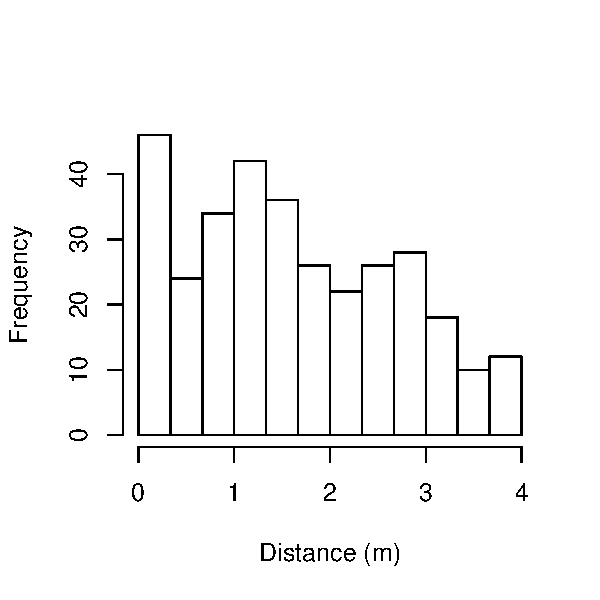
\includegraphics{intro/figs/ds-golftee.pdf}\\
\caption{A histogram of line transect data. In this case from an experiment conducted at the University of St Andrews. 760 golf tees were randomly distributed over a 1680m$^2$ area, then observed in 11 transects by 8 independent surveys. Further detail may be found in \citeb[p. 140]{ADS} and \citeb{yellowbook}.}
\label{ds-lt-example}
\end{figure}

\subsection{Point transects}
Line transects are not the only way of collecting data for a distance sampling analysis; point transects may also be used. When using point transects the observer stands at one of a series ($m$, say) of points and observes the objects surrounding him/her. Again, distances to the objects ($r_i$) are recorded. An \textit{effective radius} ($\rho$) is then calculated (analogously to $\mu$) and then object density can be written as:
\begin{equation*}
\hat{D}=\frac{n}{m \pi \hat{\rho}^2}=\frac{n}{m\pi w^2\hat{p}}.
\end{equation*}
The relation between these quantities will be explained below in \secref{gtoD}.

An example of point transect data is given in figure \ref{ds-pt-example}. In contrast to the line transect case, there are very few observations near 0, they increase to a point and then fall off beyond that. Note that as the distance, $r$, from the observation point increases the area surveyed increases as $r^2$. Rescaling this histogram by the distance to the midpoints of each bin will give a histogram that has a similar shape to that of figure \ref{ds-lt-example} (i.e. the rescaling accounts for the increasing area available to the observer as the distance from the point increases).

% example of point transect data
\begin{figure}
\centering
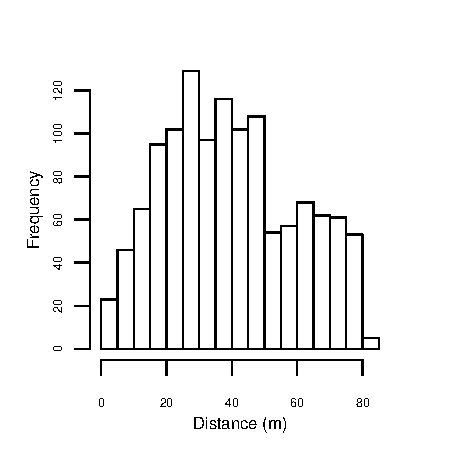
\includegraphics{intro/figs/pt-data-example.pdf}\\
\caption{A histogram of point transect data of Hawaiian amakihi (\textit{Hemignathus virens}) taken from \citeb{amakihi}.}
\label{ds-pt-example}
\end{figure}


\section{Assumptions}
In order to ensure that estimation is unbiased several assumptions are made. These are summarised below, more information (especially with regard to field procedure) may be found in \citeb{IDS}, chapter 2. The assumptions are given in order of importance from most to least.
\begin{itemize}
	\item The survey must be performed and designed properly and field procedure followed. No amount \textit{post hoc} of analysis can correct for this.
	\item Objects are distributed according to some stochastic process throughout the area of interest.
	\item Lines and points are randomly placed (with respect to the population) and a sample of $n$ objects are detected, measured and recorded. This could be via a grid with a baseline randomly placed with respect to the survey area.
	\item Objects on the line (or point) are detected with probability 1.
	\item Objects are observed in their initial location, not after movement in response to the observer.
	\item The recorded distances are accurate.
	\item Objects are correctly identified.
\end{itemize}

\section{The detection function}
\label{intro-ds-detefct}

One would expect that the probability of observing an animal would decrease as the distance from the observer increased (as in figures \ref{ds-lt-example}). This is the relationship captured by the detection function ($g(x)$) which is defined as (\cite[p. 10]{IDS}):
\begin{equation*}
g(x)=\mathbb{P} (\text{object detected} | \text{object was at distance } x).
\end{equation*}
The goal in distance sampling is to accurately model the detection function. Before talking about models for $g(x)$, we look at the desirable properties.

First, as stated in the assumptions above, objects on the line (or point) are detected with certainty, so $g(0)=1$. Second, it is preferable to have a model where detection is almost certain near zero distance, i.e. that the function has a \textit{shoulder}. This is physically realistic since the observer should see most things close to him/her (not just those directly under/in front of him/her). Third, it is also desirable that the model for the detection function is robust, in the sense that it is a general, flexible model that can take many plausible shapes (see \cite[p. 41]{IDS}). Finally, it is desirable to have a model that is efficient, in the sense that estimates have a relatively small variance, however this is only of use when the other criteria are met.

\citeb{buckland92} gives a ``key function plus adjustment terms'' formulation for the detection function. In this formulation the key function is used as a starting point for the basic shape of the detection function (it has certain detection at zero distance and has a shoulder). The adjustment terms consist of a series expansion that improve the fit of the model. The adjustment terms may not always be necessary, in which case they may be omitted from the model. The key function is usually selected as one of a uniform, half-normal or hazard-rate (\cite{buckland85}) function. The adjustment terms are typically either even simple polynomials, Hermite polynomials or cosine functions. Further information can be found in \citeb[p. 47]{IDS}. Figure \ref{ds-detfct-examples} shows some possible detection functions.

% Possible detection functions
\begin{figure}
\centering
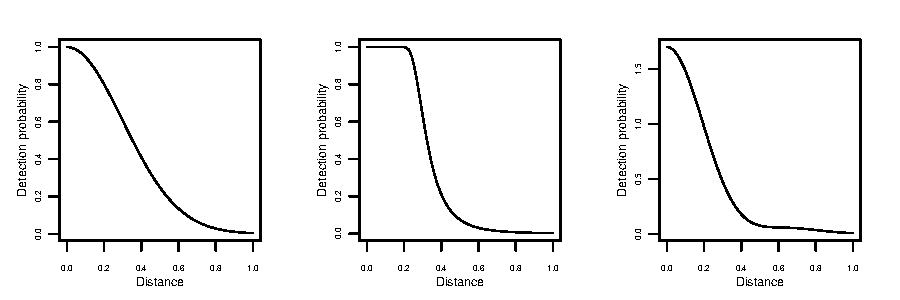
\includegraphics{intro/figs/detfct-examples.pdf}\\
\caption{Three possible detection functions. The first is a half-normal distribution, the second a hazard-rate function and the third the same half-normal as the first but with a cosine adjustment term. The hazard-rate function has a controllable ``shoulder''.}
\label{ds-detfct-examples}
\end{figure}

This formulation leads to a class of highly flexible models. Data analysis usually consists of running models made up of various combinations of key functions and adjustment terms. Model parameters are found using maximum likelihood (see \secref{gtoD}). Model selection is performed via AIC (\cite[p. 69]{IDS}), that is:
\begin{equation}
\text{AIC} = -2 l + 2P,
\label{DEFN-AIC}
\end{equation}
where $l$ is the value of the log-likelihood at the MLE and $P$ is the number of parameters in the model. Models with many parameters are penalized more heavily than those which are more parsimonious.

\section{From $g(x)$ to $D$}
\label{gtoD}
Equation (\ref{ds-D}), above shows that in order to estimate the density of the population in question, we must find an estimator of $\mu$, the effective strip width (or, equivalently for point transects, $\rho$). To do this the detection function is used.

\subsection{Line transects} 
As mentioned above, $\mu$ is defined to be the distance from the lines for which as many objects are detected beyond $\mu$ as are missed within $\mu$ (\cite{eenviron}). Looking at figure \ref{ds-mu-explanation}, the shaded area above the detection function represents those objects that the observer missed up to a distance $\mu$ from the line. The shaded area below the curve represents those objects that were observed beyond a distance $\mu$. By moving $\mu$ to the left or to the right, it is possible to find a point at which the two shaded areas are of equal size. This fulfils the criterion for $\mu$.

% explanation of mu
\begin{figure}
\centering
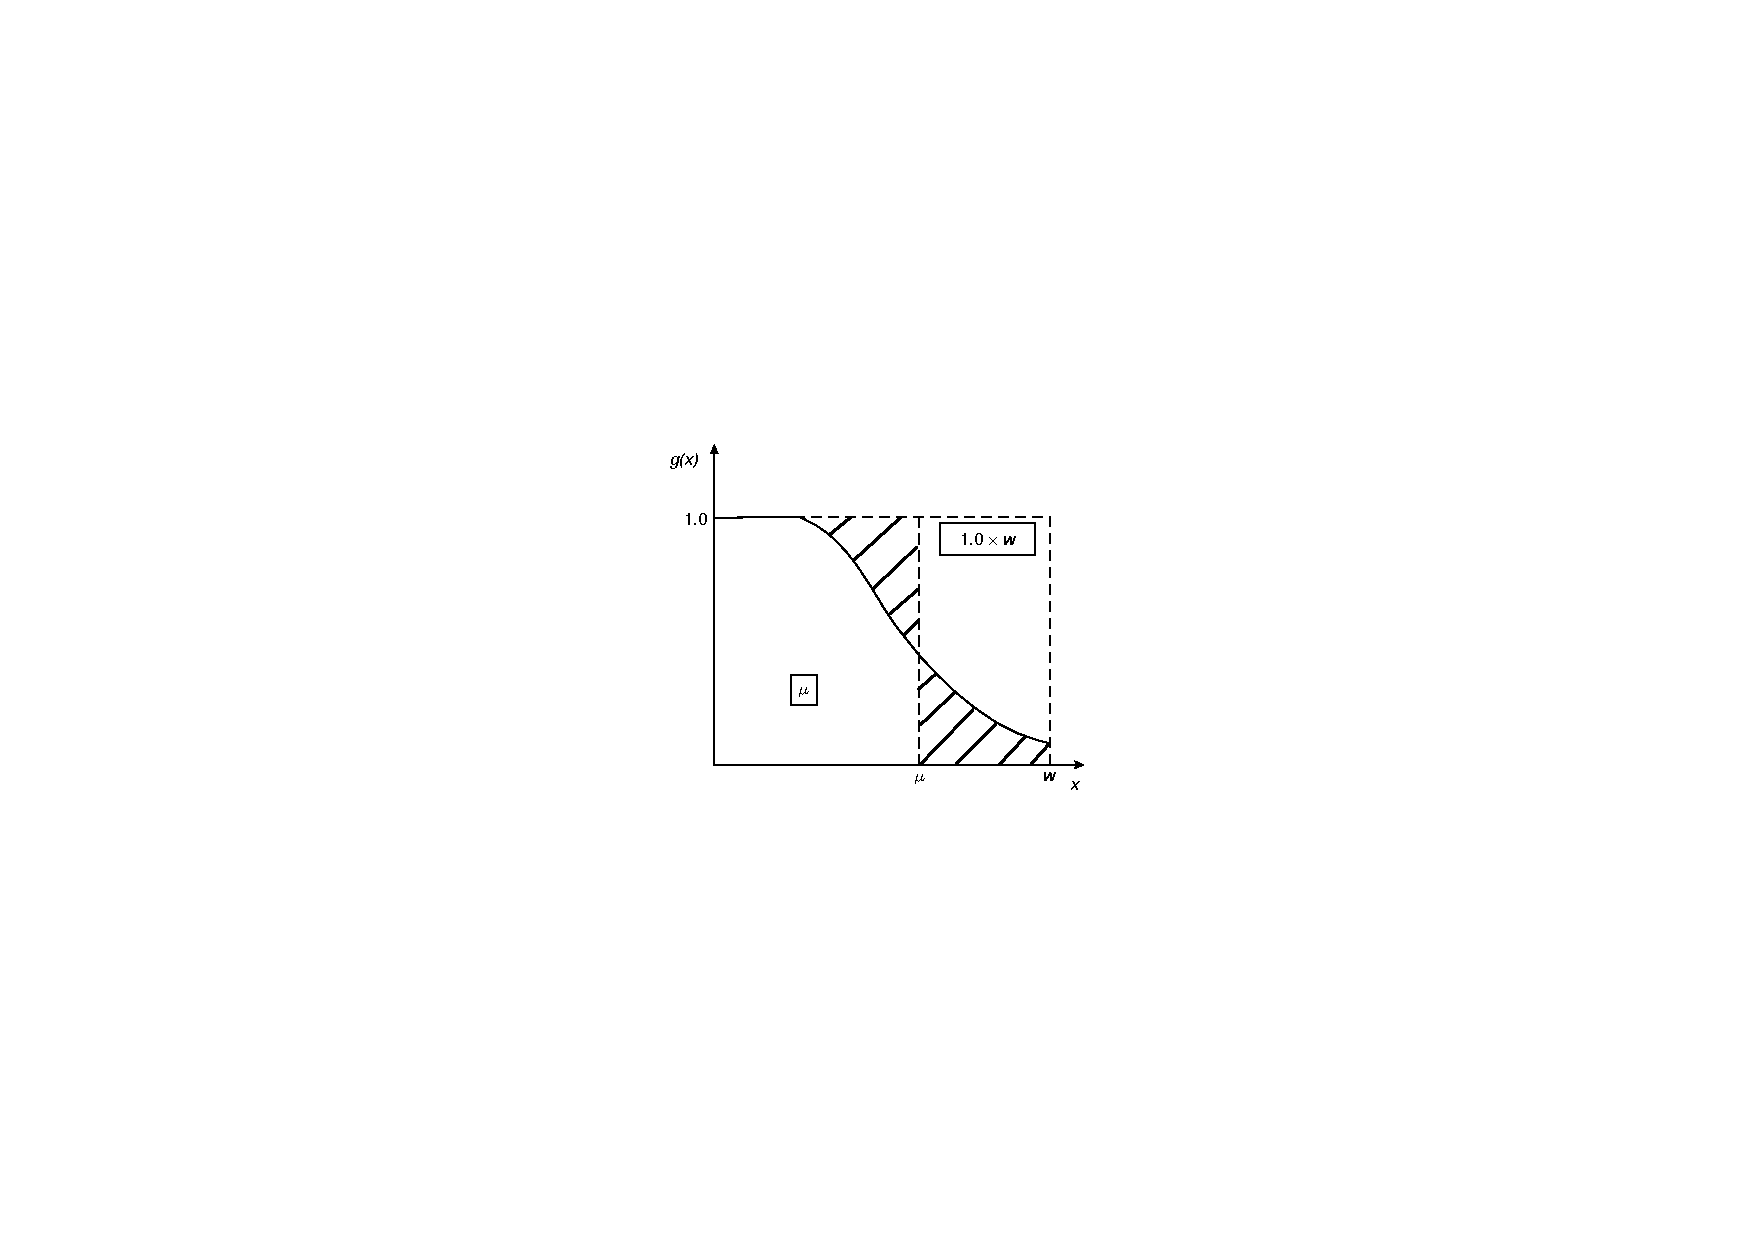
\includegraphics{intro/figs/muexplanation.pdf}\\
\caption{A detection function ($g(x)$) with the effective strip width ($\mu$) marked as well as the truncation distance ($w$). The shaded regions have equal area, this means that the area under the curve has the same size as the rectangle with base length $\mu$. Figure taken from \cite{IDS}.}
\label{ds-mu-explanation}
\end{figure}

Now the question is: how is $\mu$ calculated and how does this relate to the detection function? Note that the rectangle with side $0$ to $1$ on the $y$ axis and $0$ to $\mu$ on the $x$ axis has area $\mu$ and that this is the same as the area under the detection function (by the argument above). So, $\mu$ can also be thought of as the distance out to which the observer sees everything and is defined as:
\begin{equation}
\mu = \int_0^w g(x) \text{d}x.
\label{ds-lt-mu-def}
\end{equation}
where $w$ is again the truncation distance and ignoring the exact form of $g(x)$. Hence $p$ is defined as:
\begin{equation*}
p = \frac{\int_0^w g(x) \text{d}x}{w}.
\end{equation*}
So an estimator of density may be written as:
\begin{equation*}
\hat{D}=\frac{n}{2L \int_0^w \hat{g}(x) \text{d}x}.
\end{equation*}
The detection function is one of the functions described in \secref{intro-ds-detefct} and so only its parameter(s) must be estimated ($\bm{\theta}$, say). However to first form the likelihood, the probability density function must be defined. Note that the expected number of objects at a distance $x$ from the transect line (including those not observed) is independent of $x$. This then implies that the shape of the density functions is the same as that of the detection function and can therefore be obtained by rescaling (\cite[p. 38]{IDS}). So, the PDF of the perpendicular distance data, conditional on the object being observed is then:
\begin{equation*}
f(x;\bm{\theta}) = \frac{g(x;\bm{\theta})}{\int_0^w g(x;\bm{\theta}) \text{d}x} = \frac{g(x;\bm{\theta})}{\mu}.
\end{equation*}
%As an aside, note that by the assumption, above, $g(0;\bm{\theta})=1$, so:
%\begin{equation}
%f(0;\bm{\theta}) = \frac{g(0;\bm{\theta})}{\int_0^w g(x;\bm{\theta}) \text{d}x} = \frac{1}{\mu}.
%\end{equation}
Now we have obtained an expression for the pdf, we can form a likelihood:
\begin{align}
\mathcal{L}(\bm{\theta}; \bm{x}) &= \prod_{i=1}^n f(x_i;\bm{\theta}),\notag \\
&= \prod_{i=1}^n \frac{g(x;\bm{\theta})}{\mu}.
\label{ds-lt-likelihood}
\end{align}
The log-likelihood can then be used as an objective function in an optimization procedure in order to find the maximum likelihood estimators of the parameters.

\subsection{Point transects} 

Point transects follow an analogous explanation to line transects. Instead of effective strip width, we look at effective radius. This effective radius, $\rho$ is defined in the same way as $\mu$: that there are as many objects missed within $\rho$ as observed beyond. Related to the effective radius is the \textit{effective area of detection}, $\nu=\pi \rho^2$.

For line transects, an infinitesimal strip has area $L\text{d}x$ (that is the length of the line, multiplied by an infinitesimal distance perpendicular to the line) and this value is independent of $x$. However, in the point transect case an incremental annulus depends on $r$ (the distance from the point), such an annulus has area $2\pi r \text{d}r$. So, the effective area of detection is therefore defined as:
\begin{equation*}
\nu = 2 \pi \int_0^w r g(r) \text{d}r.
\end{equation*}
Then, following through the arguments above, we can define the PDF as:
\begin{equation*}
f(r) = \frac{r g(r)}{\int_0^w r g(r) \text{d}r},
\end{equation*}
and hence: 
\begin{equation*}
f(r) = \frac{2 \pi r g(r)}{\nu},
\end{equation*}
a more rigorous proof of this is given in \citeb[p. 54]{IDS}.

By analogy to the line transect case the relation between $\nu$ and $p$ in the point transect case is
\begin{equation*}
p=\frac{\nu}{\pi w^2}
\end{equation*}
so
\begin{equation*}
f(r) = \frac{2 \pi r g(r)}{\pi w^2 p}.
\end{equation*}
So again, a likelihood can be formed:
\begin{align*}
\mathcal{L}(\bm{\theta}; \bm{r}) &= \prod_{i=1}^n f(r_i;\bm{\theta}),\\
&= \prod_{i=1}^n \frac{2 \pi r g(r;\bm{\theta})}{\nu}.
\end{align*}
As above, the log of this expression can then be used in an optimization procedure to find the MLEs of the parameters.


\section{Multiple covariate distance sampling}
\label{intro-ds-covar}

One can very easily think of the case in which one or more factors affect the detectability of objects in a survey as well as distance. A typical example might be sex or size of the object or weather conditions during when the object was observed. When available this information can be very useful in handling heterogeneity in the data (\cite[p. 88]{IDS}). Covariates are included in detection function models by using a link function. The parameter(s) of the detection function can be considered to be a linear combination of the covariates. Figure \ref{ds-covarex} shows the effect of both continuous and factor covariates on a hazard-rate detection function.

% example covariates and how they effect the detection function
\begin{figure}
\centering
% trim order l b r t
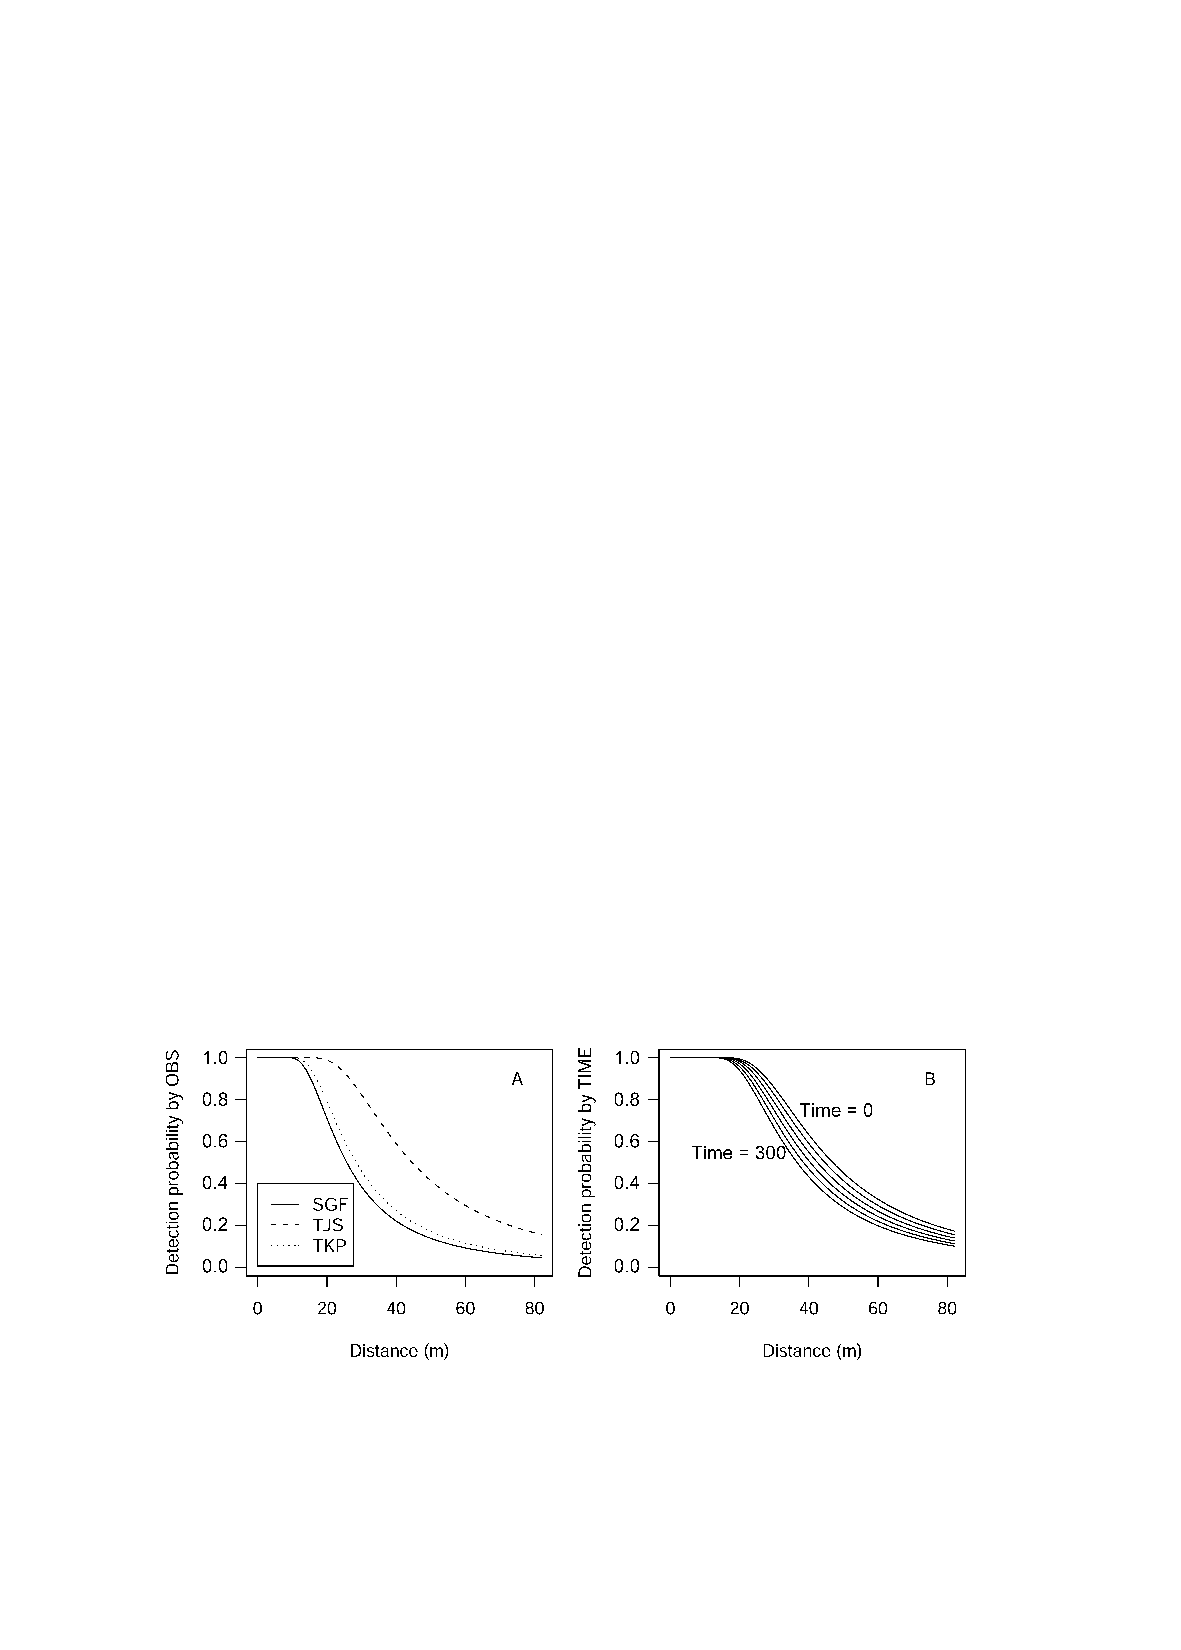
\includegraphics{intro/figs/amakihi-detfct.pdf}\\
\caption{The influence of covariates on the detection function (taken from \cite{amakihi}). The detection functions are for Hawaiian amakihi (\textit{Hemignathus virens}). The left panel shows the effect of a factor covariate (observer), while the right shows the effect of a continuous covariate (time). In each case the other covariate is held constant (time at $0900$ and observer as ``TJS'', respectively) while the other is varied.}
\label{ds-covarex}
\end{figure}

Considering a detection function modelled by a half-normal, $g$ is written as:
\begin{equation*}
g(x; \sigma) = \exp\left (\frac{-x^2}{2\sigma^2}\right ),
\end{equation*}
now, say that two covariates have been collected, $z_{i,\text{sex}}$ and $z_{i,\text{Beau}}$ indicating the sex of animal $i$ and the Beaufort sea state when animal $i$ was observed. Also recorded are the distances $x_i$. Covariates can be included in the analysis by considering $\sigma$ as a linear combination of these covariates:
\begin{equation}
\sigma_i = \exp( \beta_0 + \beta_1 z_{i,\text{sex}} + \beta_2 z_{i,\text{Beau}}),
\label{intro-ds-beaufort-covar-model}
\end{equation}
The objective is now obtaining estimates of $(\beta_0, \beta_1, \beta_2)$.

More generally one can of the covariates $\mathbf{z}$ (a $K$-vector of $z_1, \dots, z_K$) related to the observation $x$. The complete set of covariates for all observations is stored in $\mathbf{Z}$, an $n \cross K$ matrix. The scale function is indexed by $i$ when covariates are used, so the more general form of (\ref{intro-ds-beaufort-covar-model}) is:
\begin{equation}
\sigma_{i} = \exp( \beta_{0} + \sum_{k=1}^K \beta_k z_{ik}).
\label{intro-ds-covar-model}
\end{equation}

This covariate formulation can be thought of as a generalisation of the non-covariate model, the latter simply being the case where there is only an intercept term. 

This formulation fits nicely into the likelihood expressions above, the evaluations of the detection function are as above, but the calculation of $\mu$ (and therefore $p$) changes. 

The effective strip width, $\mu_i$ is now expressed as:
\begin{equation}
\mu_i = \int_0^w g(x ; \sigma_i) \text{d}x,
\label{intro-ds-mu-covar}
\end{equation}
that is, that the effective strip width depends on the covariate values. So in the covariate case there is no single probability of detection, instead the per observation (equivalently, per unique covariate combination) probability of detection can be calculated for line transects:
\begin{equation*}
p_i = \frac{\int_0^w g(x ; \sigma_{i}) \text{d}x}{w}.
\end{equation*}
For point transects, the probability of detection and effective area are given as:
\begin{equation*}
p_i =\frac{2}{w^2}\int_0^w r g(r; \sigma_i) \text{d}r, \qquad \nu_i = \int_0^w r g(r; \sigma_i) \text{d}r.
\end{equation*}

\subsection{Estimating population size}
\label{intro-ds-pop-size}

Population size can be found either by multiplying $D$ by the survey area or from a Horvitz-Thompson-like estimator (\cite[pp. 53-56]{thompson}, \cite[p. 23]{ADS}).

For the covariate models this is:
\begin{equation}
N = \sum_{i=1}^n \frac{1}{c_i p_i},
\label{HT-ds-est}
\end{equation}
where $c_i$ is probability of the $i^\text{th}$ observation being within the sampled area, and $p_i$ is the probability of the $i\text{th}$ observation being detected given it is within the sampled area (\cite[p. 38]{ADS}).  

For non-covariate models, this simplifies to:
\begin{equation}
N = \frac{n}{p},
\end{equation}
if the probabilities of the observation being in the sampled area are all the same (\cite[p. 10]{ADS}).

A standard summary statistic is the \textit{average detection probability} for an animal within the covered region, $P_a$, which is given by:
\begin{equation*}
P_a = n/N.
\end{equation*}

\section{Other considerations}

\subsection{Line and point placement}
The placement of the lines and points above is said to be ``random'', in practise randomly placing and orientating lines can be expensive and time-consuming (in particular in shipboard surveys where one wishes to minimise off-effort time). The solution to this is simply randomly placing and orientating a grid of lines or points (\cite[p. 2]{IDS}). For shipboard surveys ``zigzag'' designs can be used to minimise off-effort time (\cite{strindberg04}). It is also important to ensure that transects to not run parallel to geographical features as doing this will incur bias. For example using roads as transects (as was done in the US breeding bird survey) leads to bias since animals may be compelled to move away from the road and toward neighbouring hedgerows (\cite[p. 18]{IDS}).

\subsection{Clusters}
If animals are observed in clusters (for example pods for whales or packs for wolves) then it might be more convenient to estimate the abundance of clusters and use them as the fundamental unit to estimate. The cluster size can also be estimated and the abundance of clusters ``multiplied up'' to give the overall abundance (\cite[p. 13]{IDS}). It is assumed throughout that individuals rather than clusters are being addressed but the method developed here should also work on clusters.

\subsection{Goodness of fit testing}
Although AIC is a good measure of relative fit of a model, some formal absolute measure of goodness of fit is also useful (the best of a bad lot is still bad). $\chi^2$ testing has been suggested (\cite[pp. 69-71]{IDS}), however the choice of interval is subjective. As a replacement, Kolmogorv-Smirnov and Cramer-von Mises tests (\cite[pp. 385-389]{ADS}) are suggested. Both are used to compare empirical to cumulative distribution functions (EDFs and CDFs, respectively). The Kolmogorov-Smirnov test uses the largest difference between the fitted CDF and the EDF as a test statistic, with the null hypothesis that the functions are the same. The Cramer-von Mises test has the same null hypothesis but the test statistic is instead based on the differenced between the CDF and EDF over their entire range.

\section{Summary}
Distance sampling is unlike many statistical methods, in that the quantity which we wish to find, abundance, is not given explicitly in the likelihood we wish to optimize. Instead we wish to find the parameters for the detection function, to then estimate of $\mu$, in order to estimate density (and hence the abundance). Full likelihood methods for distance sampling require that probabilistic models for the animal distribution be specified which may well be very tricky. CDS and MCDS specify probability models only for the distance parts of the data and then assume $\log$-normality for variances and confidence intervals for $\hat{N}$. Although this means that estimators do not have  properties such as asymptotic efficiency, they do avoid the specification of the animal distribution or, for MCDS, the joint distribution of the covariates and distribution (see \cite[p. 6 and pp. 31-33]{ADS}). Contrasting this with capture-recapture, where the abundance is obtained directly from finding the MLE of the parameters, it seems rather complex and esoteric. 

Distance sampling benefits from a relatively simple field procedure, a wealth of literature and easy to use software for analysis. Distance sampling has also been adapted for many different scenarios, including analysing data which was not initially part of a survey (incidental data).

Non-covariate distance sampling, as described above, is commonly referred to as CDS (conventional distance sampling) and covariate distance sampling as MCDS (multiple covariate distance sampling. Other variants exist, for example mark-recapture distance sampling (MRDS, \cite{mrdspaper}) and spatial distance sampling models (\cite[chapter 4]{ADS}).

\section{Monotonicity}
\label{intro-ds-mono}
One potential pitfall of both CDS and MCDS is that  it is possible to formulate models which are not physically realistic. In particular it is possible to create models for the detection function which are non-monotonic functions of distance. Data with a mode away from zero distance may occur when there has been heaping (when observers ``eyeball'' distances and round to convenient numbers like 5, 10, 20m etc, \cite[pp. 34-35]{IDS}), when objects move prior to observation or just by chance. Fitting models to such ``bumps'' can cause bias in abundance estimates (\cite[p. 132]{IDS}). To get around this problem \citeb{distance-software} constrains the detection function to be monotonic. This is done by taking 10 equally spaced distances from $0$ to $w$ and checking that when the detection function is evaluated at each of these points they are less than the last ($g(x_i)\geq g(x_{i+1})$ for distances $x_1 \dots x_{10}$ where $x_1=0$). This is referred to as \textit{strong monotonicity}. Alternatively, \textit{weak monotonicity} may be enforced, where each point is checked only against the value of $g$ at the origin ($g(0)\geq g(x_i)$).

Constrained optimization is appealing here, however it is obviously always preferable to perform unconstrained optimization if possible. Using a class of functions to model the detection function which were both flexible and did not exhibit the undesirable property of non-monotonicity could offer a more physically realistic and convincing alternative to the conventional way of performing distance analyses.

Although constraining the shape of the detection function is possible, it does not necessarily lead to monotonic detection functions since the constraints can only be applied at a finite number of points. This can lead to constraints missing the non-monotonic points in the function. An example from \citeb{williams} is shown in the first panel of figure \ref{fig1}. Here a half-normal detection function was fit with one second order cosine adjustment term to humpback whale sightings. The second and third panels in figure \ref{fig1} show a detection function when covariate data was included in the model. In this case for long-finned pilot whales (\cite{pike}) the Beaufort sea state was added as a covariate, the first plot shows that the detection function, when averaged over the covariate values, shows some non-monotonic behaviour. However, in the third panel the marginal detection function at 25\%, 50\% and 75\% quantiles of the covariate are shown and here the non-monotonicity is particularly pronounced. Given the above, a formulation that guarantees monotonicity from the outset is appealing.

\begin{figure}
\centering
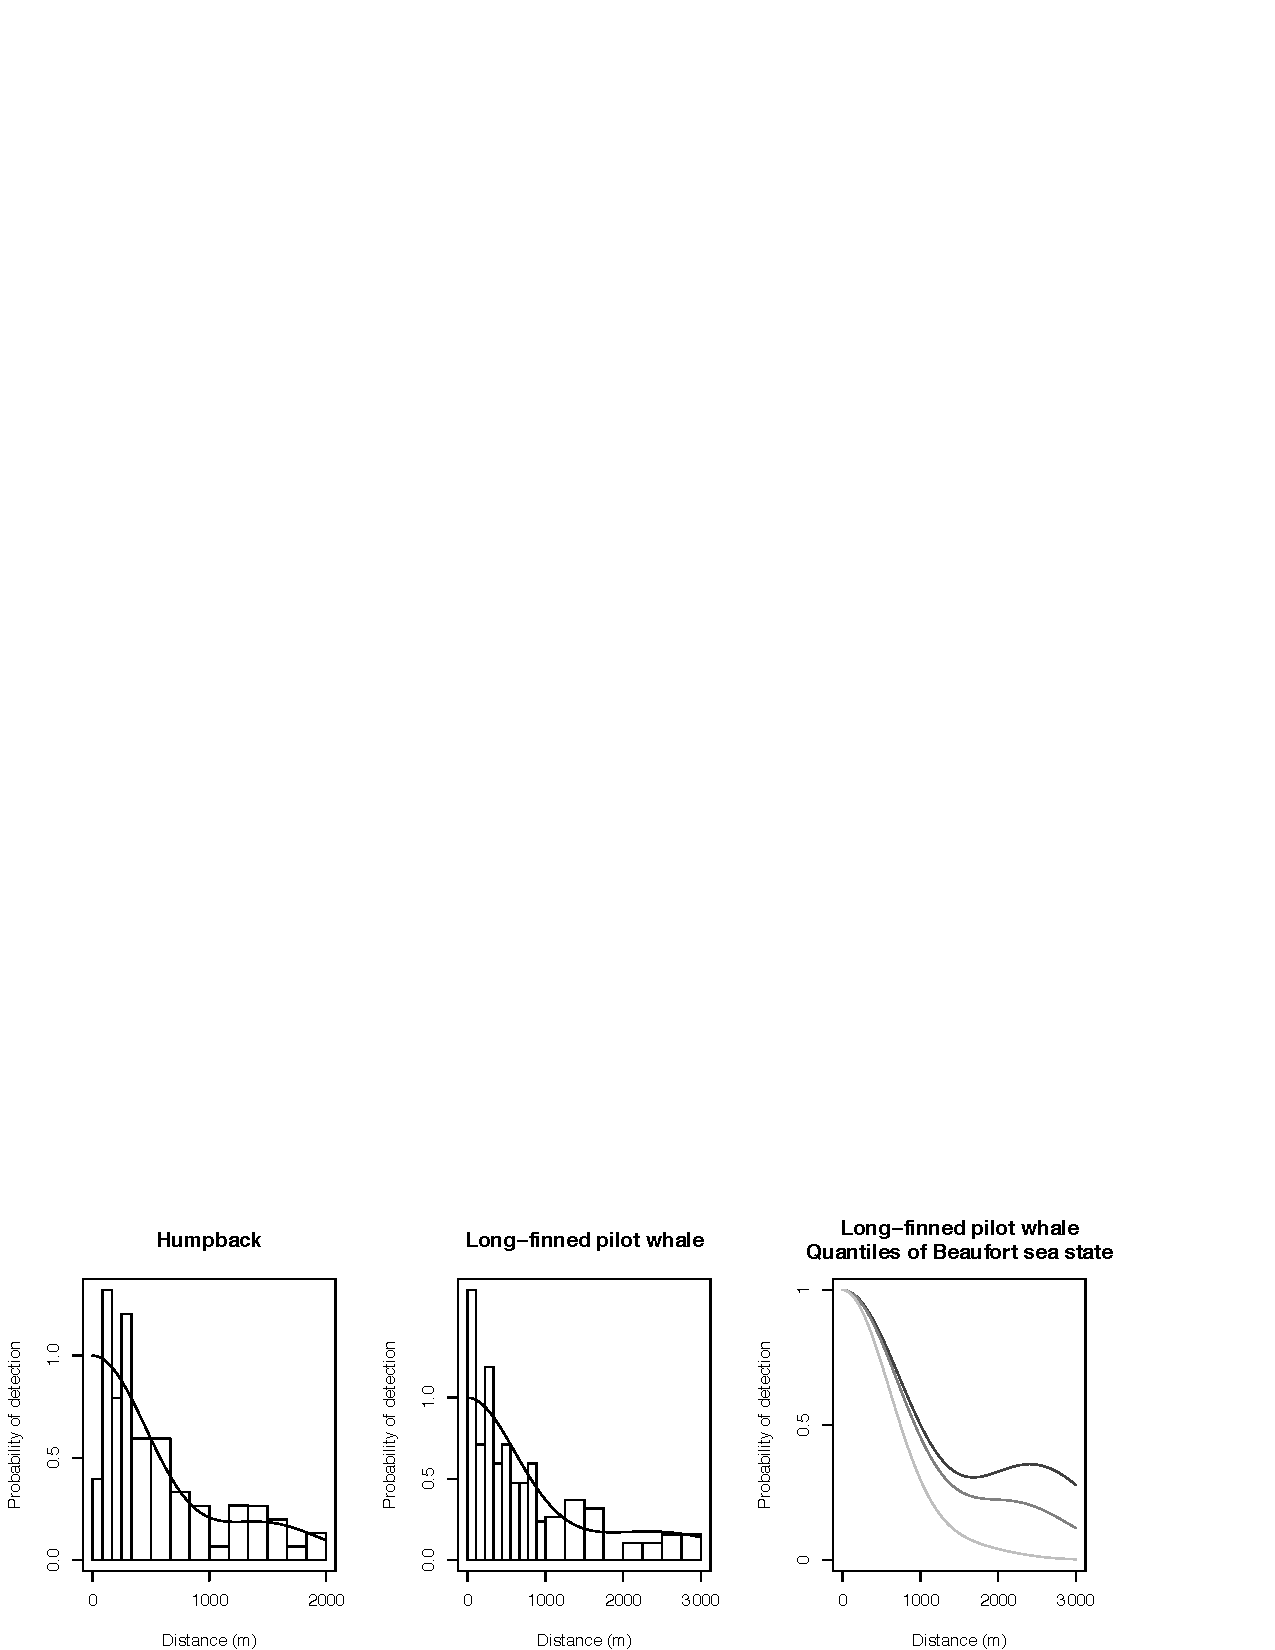
\includegraphics[width=\textwidth]{mix/figs/figure1.pdf}
\caption{Two examples of detection functions which are not monotone. The first first panel is data from humpback whale (reproduced from data in \citeb{williams}), a half-normal detection function with cosine adjustments provided the best fit to the data, even with constraints in place, the detection function is non-monotonic. The second and third panels are plots for the long-finned pilot whale data taken from \cite{pike}. In the second panel the detection function is averaged over the covariate values and the third shows marginal detection function for quantiles of the Beaufort sea sate covariate (the model was a half-normal detection function), showing that the non-monotonicity gets worse at higher levels of the covariate.}
\label{fig1}
\end{figure}

\section{Mixture models}

Recently developments, particularly in mark-recapture (\cite{pledger2000}, \cite{dorazio03}, \cite{pledger2005} and \cite{morgan08}) have shown that mixture models can be an extremely useful and flexible method of modelling heterogeneity in biological populations. Their main utility has been in better accounting for between-individual heterogeneity which can cause severe bias if unmodelled (\cite{Link2003}). 

In distance sampling bias due to unmodelled heterogeneity is not severe unless the heterogeneity is extreme (\cite[pp. 389-392]{ADS}) and provided that the detection at zero distance is certain and a flexible detection function model is used. So called \textit{pooling robustness} allows abundance estimates of the whole population to have low bias (although abundance estimates of subpopulations, e.g. males or females alone, may be biased). As noted in \citeb[pp. 391]{ADS} it is important that the model used for the detection function is sufficiently flexible to accommodate the detection functions resulting from pooling data. Mixture models offer the potential for flexible modelling in this way and also have the appealing property that if the individual parts of the mixture model (the mixture components) are each monotonic decreasing then a sum of these functions will also be monotonic decreasing. Each constituent component of the mixture model is simple but the combinations yield a great many possible shapes (see figure \ref{sim-detfcts}), while at the same time constrained optimization is avoided.

%Covariates provide some information on those factors which may effect the detectability of individuals, modelling some of the heterogeneity in the detection process. Adjustment terms attempt to perform a similar task (though in an admittedly blunter fashion) by smoothing the function of distance in a semi-parametric way. A combination of the two approaches is possible although some have philosophical opposition to it (Jeff Laake, personal communication). One would like to both handle heterogeneity with both the data at hand (in the form of covariates) whilst also ``smoothing away'' residual effects of unobserved states in the population (while maintaining monotonicity).

Finally, the approach is also interesting for its own sake. There is no current literature on the use of mixture models as detection functions for distance sampling. Many detection function forms have been proposed (\cite{buckland92} and  \cite{gammadetfct}), each having their own merits and pitfalls. Therefore, there may be useful and unexplored properties of using a mixture model for the detection function that have not been previously considered.

A mixture model approach to distance sampling detection functions is developed further in the next chapter.

\section{Acknowledgement}

This part of the thesis is based on the paper ``Mixture models for distance sampling detection functions'' by the author and Len Thomas of the Centre for Ecological and Environmental Modelling at the University of St Andrews and is in preparation to submit to Biometrics. A mixture model approach to line transect detection functions without covariates was developed as part of the author's MMath thesis at the University of St Andrews under the supervision of Len Thomas. The material detailed here is a significant development from the methods developed in that thesis.

